\documentclass[12pt,fleqn,a4paper,oneside]{LegrandOrangeBook}
\addbibresource{sample.bib} % Bibliography file
\definecolor{ocre}{RGB}{103, 61, 76}
\chapterimage{orange1.jpg} 
\chapterspaceabove{6.5cm}
\chapterspacebelow{6.75cm} 
%\begin{theorem}[Name of the theorem]
%\begin{exercise}
%\begin{example}[Example name]
%\begin{definition}[Definition name]
%\begin{corollary}[Corollary name]
%\begin{remark}
%\begin{proposition}[Proposition name]
%\begin{problem}
%\begin{vocabulary}[Word]
%\begin{notation}
%----------------------------------------------------------------------------------------
\begin{document}
%----------------------------------------------------------------------------------------
%----------------------------------------------------------------------------------------
%Lineas
%----------------------------------------------------------------------------------------
\section{Leyes de maxwell}\index{Leyes de maxwell}
Se presentan las ecuaciones de Maxwell en la tabla \ref{tab:maxwell}.
\begin{table}[]
\begin{tabular}{|l|l|l|}
\hline
\rowcolor[HTML]{0066cc} 
Forma diferencial & Forma integral                                                                 & Comentario\\ \hline
$\nabla\cdot \textbf{D}=\rho_v$  & $\oint_S\textbf{D}\cdot d\textbf{S}=\int_v\rho_vdv                                 $ & Ley de Gauss\\ \hline
$\nabla\cdot \textbf{B}=0$ & $\oint_S\textbf{B}\cdot d\textbf{S}=0
$ & No existencia de monopolos \\ \hline
$\nabla\times \textbf{E}=-\frac{\partial \textbf{B}}{\partial t}$    & $\oint_L\textbf{E}\cdot dl=-\frac{\partial}{\partial t}\int_S\textbf{B}\cdot dS
$ & Ley de Faraday\\ \hline
$\nabla\times \textbf{H}=\textbf{J} + \frac{\partial \textbf{D}}{\partial t}$ & $\oint_L\textbf{H}\cdot dl=\int_S\left(\textbf{J} + \frac{\partial \textbf{D}}{\partial t}\right)\cdot d\textbf{S}$ & Ley de circuitos de Ampere \\ \hline
\end{tabular}
\caption{Leyes de Maxwell}
\label{tab:maxwell}
\end{table}
Donde es necesario recordar el operador DEL (\ref{subsec:DEL})
\begin{itemize}
\item El gradiente de un escalar V: $\nabla$V
\item La divergencia de un vector A: $\nabla\cdot$A
\item La rotacional de un vector A: $\nabla\times$A
\item El Laplaciano de un escalar V: $\nabla^2$V
\end{itemize}
Además se tienen ecuaciones auxiliares:
\begin{subequations}
\begin{align}
\intertext{Relación entre la Densidad de Campo Eléctrico y la Intensidad de Campo Eléctrico.}
\textbf{D}&= \epsilon \textbf{E}\\
\intertext{Relación entre la Densidad de Campo Magnético y la Intensidad de Campo Magnético.}
\textbf{B}&=u\textbf{H}\\
\intertext{Densidad de Corriente de conducción.}
\textbf{J}&=\sigma\textbf{E}\\
\intertext{Densidad de Corriente de convección en función de la densidad de carga volumétrica.}
\textbf{J}&=\rho_v\textbf{v}
\end{align}
\end{subequations}
Hay ligeras modificaciones si son para conductores malos (aislantes):
\begin{subequations}
\begin{align}
\textbf{D}&= \epsilon \textbf{E} + P\\
\textbf{B}&=u(\textbf{H} + M)
\end{align}
\end{subequations}
Donde P es el campo de polarización y M es el campo de magnetización, cuando el dieléctrico es lineal se tiene:
\begin{align*}
&P=\chi_e\epsilon_0\textbf{E} &M=\chi_m\textbf{H}
\end{align*}
\begin{figure}[H]
\centering
\subfloat[Ecuación de onda para campos eléctricos.]{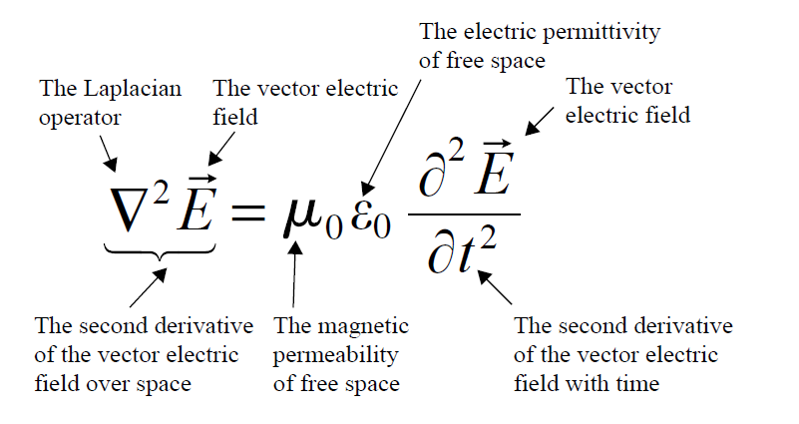
\includegraphics[width=0.8\linewidth]{LT/LT1.png}}\\
\subfloat[Ecuación de onda para campos magnéticos.]{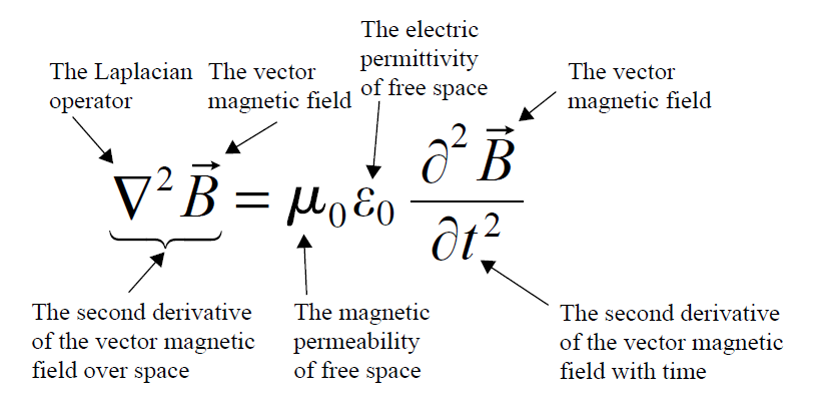
\includegraphics[width=0.8\linewidth]{LT/LT2.png}}
\caption{Ecuaciones de onda}
\end{figure}
%\section{Modelo electromagnético y las leyes de Maxwell}
%----------------------------------------------------------------------------------------
%Internetworking
%----------------------------------------------------------------------------------------
\section{Métodos para control de la congestión}
\begin{figure}[H]
\centering
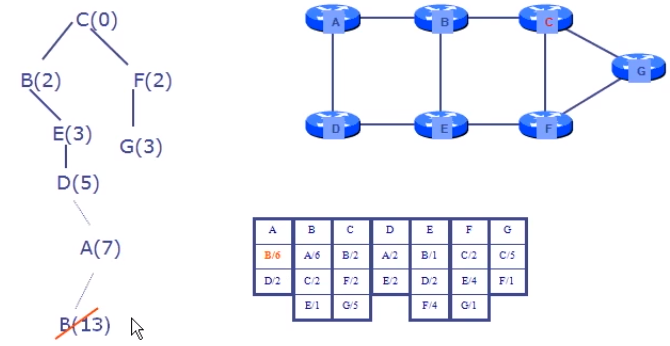
\includegraphics[width=0.8\linewidth]{IN1/IN75.png}
\caption{Escalas de tiempo de los métodos para el control de la congestión.}
\end{figure}
\subsection{Enrutamiento consiente de tráfico}
El objetivo es desviar el tráfico de los puntos más activos hacia otros, esto esta en desuso debido a su oscilación
\begin{center}
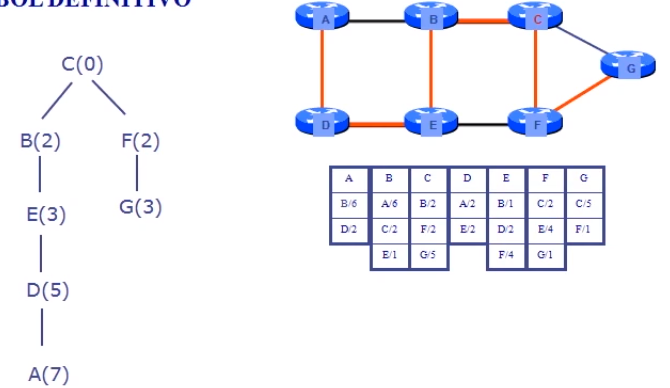
\includegraphics[width=0.8\linewidth]{IN1/IN76.png}
\end{center}
Sean dos sistemas autónomos como la image, los enlaces entre ambos sistemas son CF y EI, al congestionarse CF se enrutará los paquetes hacia EI para despejar CF. Pero luego de este proceso EI estará congestionado y verá EI como una ruta optima. El sistema de enrutamiento será \textbf{oscilatorio}.
\subsection{Regulación de tráfico}
\begin{figure}[H]
\centering
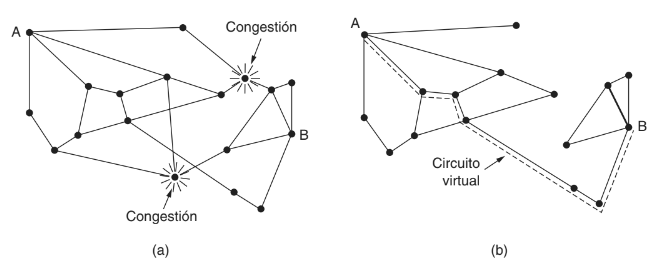
\includegraphics[width=\linewidth]{IN1/IN77.png}
\caption{(a) Una red congestionada. (b) La parte de la red que no esta congestionada.}
\label{fig:regulacion trafico}
\end{figure}
En la figura \ref{fig:regulacion trafico}.a se muestra la red con dos puntos de congestión, lo que haremos es eliminar esos puntos de congestión y calculando una nueva ruta virtual evitando los puntos de congestión. El problema puede ser que esta desviación tome un poco más de tiempo. Al existir una congestión, el router congestionado devuelve un trama al azar y envía un \textbf{paquete regulador} con un bit de encabezado al emisor para que no generé más paquetes y se reduzca el tráfico. Esto no es equitativo pues los emisor más rápidos tendrán más paquetes congestionados que lo emisores lentos.
\subsubsection{ECN}
ENC o notificación explicita de congestión, funciona similar al \textbf{paquete regulador}, en vez de crear un datagrama que vuelva al emisor, se configura dos bits para que cuando lleguen al receptor este se enteré en donde hubo una congestión y este mandará un mensaje al emisor directo para que tome las medidas.
%%22:27l
%----------------------------------------------------------------------------------------
%Microprocesadores
%----------------------------------------------------------------------------------------

%----------------------------------------------------------------------------------------
%Mantenimiento
%----------------------------------------------------------------------------------------
\part{Electrotécnia}
\chapterimage{chapter_head_Elec.pdf}
\begin{itemize}
\item libro 1
\item libro 2
\end{itemize}
\chapter{Números complejos}\index{Números complejos}
Este texto va despues
%----------------------------------------------------------------------------------------
\end{document}
%----------------------------------------------------------------------------------------
